% Use class option [extendedabs] to prepare the 1-page extended abstract.
\documentclass[extendedabs]{bmvc2k}
\usepackage[colorlinks = true,
            linkcolor = blue,
            urlcolor  = blue,
            citecolor = blue,
            anchorcolor = blue]{hyperref}
\usepackage{kotex}
% for the fancy \koTeX logo
\usepackage{kotex-logo}
\usepackage{mathtools}  % brings in amsmath, also some improvements
\usepackage{amssymb} % brings in amsfonts, incl \square
% Document starts here
\usepackage{graphicx}
\begin{document}


\title{Grad-CAM pre-report}
\addauthor{
Taehun Kim$^{1}$
}{}{1}

\addinstitution{
$^1$ Department of Computer Science and Engineering, Pusan National University.  
}
 

\maketitle
\noindent

\section{Introduction}
Class Activation Mapping(CAM)\cite{cam} modifies image classification CNN architectures replacing fully connected layers with global average pooling and a $1\times1$ convolutional layer for visual explanation. this approach cannot be applied to any other tasks except the image classification, and need to re-train. 
 
In contrast, Gradient-weighted Class Activation Mapping(Grad-CAM)\cite{gradcam} is the technique for producing visual explanations, without modifying the CNN architecture or re-training the model. Therefore this approach can be applied to various CNN model like image classification, segmentation, object detection, and image captioning.

This report summarize the Grad-CAM paper\cite{gradcam} with emphasis on its approach and architectural design.

\begin{figure}[t]
\centering
	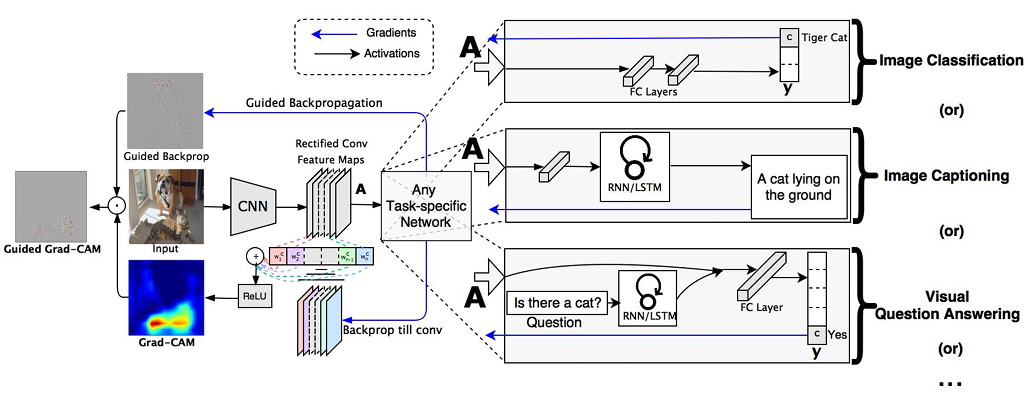
\includegraphics[width=\linewidth]{images/fig1.PNG}
	\caption{
		Grad-CAM overview}
	\vspace{-2mm}
        \label{fig:gradcamoverview}
\end{figure}

\section{Grad-CAM}
The last convolutional layer in a CNN has the best compromise between high-level semantics and spatial information. Grad-CAM uses the gradient information flowing into the last convolutional layer of the CNN. 
This method identifies the regions that contributed to the CNN's decision-making process.

Let activation maps of last convolutional layer is $A \in \mathbb{R}^{H\times W\times K}$, which $H\times W$ is resolution of the activation map and $K$ is the number of the activation maps. Let $y^c$denote the class score for class c before the softmax activation. First, The paper computes gradient of class score $y^c$ with respect to the $k$th map, $i$th column, $j$th row of $A$. Second, They apply global average pooling to the gradient to get the gradient of class score $y^c$ with respect $k$th $A$, $\alpha_k^c$:

$$
\alpha_k^c = \frac{1}{HW}\sum_{i=1}^W \sum_{j=1}^H \frac{\partial y^c}{\partial A^k_{ij}}
$$
, where the $A^k_{ij}$ is the $k$th map, $i$th column, $j$th row of activation maps of the last convolutional layer. Since $A$ is the last convolutional layer, the gradient calculation involves successive matrix multiplications of the weight matrices and the gradient with respect to activation from class score to last convolutional layer through Backpropagation(chain rule). $\alpha_k^c$ captures the importance of $k$th feature map for a target class c.

Additionally, They calculate localization map for class c using $\alpha_k^c, A^k,$ and ReLU:
$$
L^c_{Grad-CAM} = ReLU(\sum_k \alpha_k^c A^k)
$$
The product of $\alpha_k^c$ and $A^k$ highlights the significant regions within the activation map $A^k$.
ReLU is applied to retain only features with positive contributions, as negative values likely correspond to other classes.

$$
\text{ReLU}(x) =
\begin{cases} 
0 & \text{if } x \leq 0, \\
x & \text{if } x > 0.
\end{cases}
$$

\subsection{Guided Grad-CAM}
As shown in the figure \ref{fig:gradcamguidedgradcam}, Grad-CAM can localize region relevant to the class, but lacks to highlight fine-grained details. However, Guided Back-propagation\cite{guidedbackprop}, which is visualize gradient that suppress the negative gradient(and activation) during the backpropagation, capture the details of the objects, but not class-discriminative. 

The authors combine Guided Backpropagation and Grad-CAM through element-wise multiplication to integrate both information. Grad-CAM output is upsampled to the input image size for multiplication. This fusion can visualize the interesting region with high-resolution and class-discriminative.


\begin{figure}[t]
\centering
	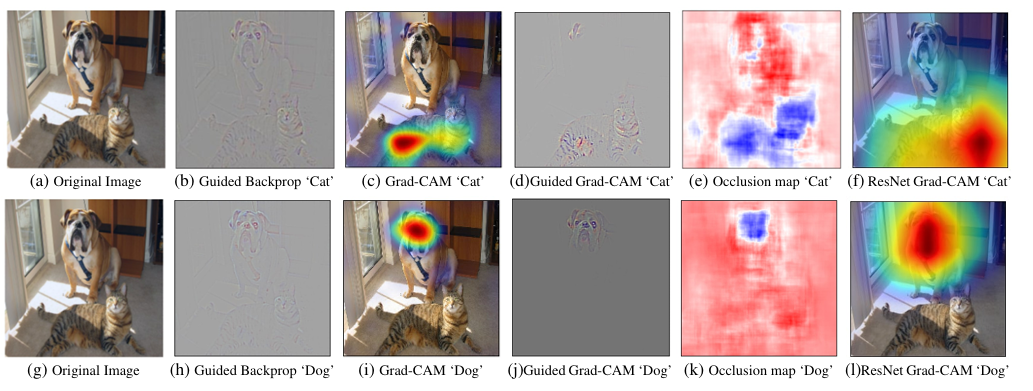
\includegraphics[width=\linewidth]{images/fig2.PNG}
	\caption{
		Guided Backpropagation, Grad-CAM, and Guided Grad-CAM}
	\vspace{-2mm}
        \label{fig:gradcamguidedgradcam}
\end{figure}

\section{Conclusion}
We summarize the Gradient-weighted Class Activation Mapping (Grad-CAM) paper \cite{gradcam}. Grad-CAM visualizes which parts of an image are important for a specific class without modifying the pre-trained model architecture or requiring re-training. 

Additionally, Guided Grad-CAM provides more precise visualizations by combining Grad-CAM with Guided Backpropagation \cite{guidedbackprop}.

\newpage
\bibliography{egbib}

\end{document}
